\documentclass[letterpaper, 10 pt, conference]{ieeeconf}
\usepackage{xcolor}
\newcommand\todo[1]{\textcolor{red}{#1}}   %I use this command to highlight areas that are unfinished
%\renewcommand\todo[1]{}   % uncomment this to hide all \todo{} in the text.
\usepackage{hyperref}
\usepackage{geometry}
\usepackage{overpic}
\graphicspath{{./pictures/pdf/},{./pictures/ps/},{./pictures/png/},{./pictures/jpg/}}
\begin{document}
\author{Shiva Shahrokhi}
\title{Literature Review on Human Interaction with Globally-Controlled Swarms}
\maketitle

\begin{abstract}

Simple robots can do huge things. To control swarm of simple robots, we need to know how to steer them simply. One way is global control which means a single input to all the robots (or particles). Previous works show that humans can do it, so we want computers to do it automatically and efficiently.
 
\end{abstract}

\section{Literature Review}
\subsection{Micro assembly using a cluster of paramagnetic Microparticles:}

In this paper, Khalil et al. use an external magnetic source to guide cluster of paramagnetic micro particles to achieve point to point positioning of the cluster, manipulation of micro objects and assembly of micro objects into a microstructure in \cite{Khalil2013}.They experimentally analyzed the relation between the number of micro particles within the cluster and its average linear velocity. They have created the micro objects on silicon wafer. Drag forces on the cluster of micro particles and micro objects are estimated using the applied current to each of the electromagnets and the velocity of the cluster. Future work is 3D controlling and 2D controlling in a better velocity.
\begin{figure}[h]
\begin{center}
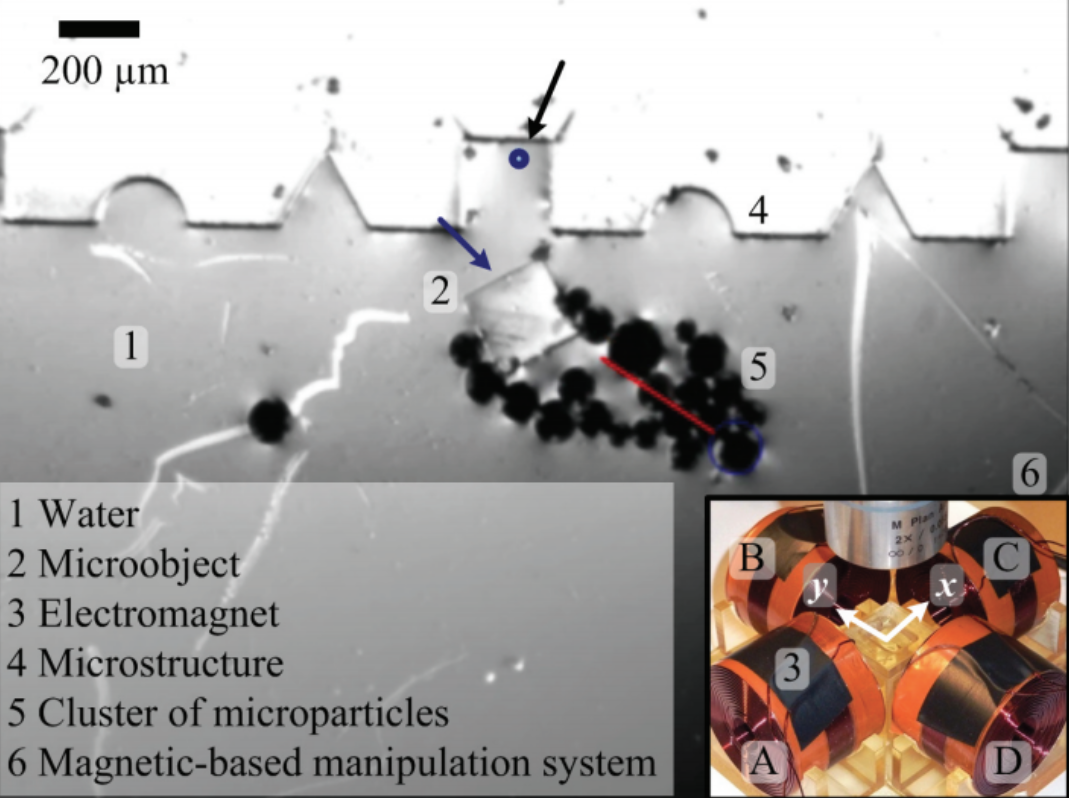
\includegraphics[width=\columnwidth]{khalil.png}
\caption{Assembly of a micro object to a micro structure using a cluster of microparticles\cite{Khalil2013}.
\label{fig:khalil}}
\end{center}
\end{figure}

\subsection{Massive Uniform Manipulation}

In this paper, Becker et al. use a common input signal to control large populations of simple robots in \cite{AaronManipulation2013}. When you want to control a swarm with a single global command, you must have at least one obstacle to control the swarm. They had three methods to work with: Addressable, Local and Global. Addressable means that each robot has its own name and the system in this state is fully controllable. Local means that each robot has a parameter to scale the turning rate and with this parameter it is completely controllable. and the third method is Global, which means all the robots get the same input, but we should have at least one obstacle to control position of all the robots. They had shown that the global command is the fastest way for humans to lead the robots to the goal position and Local is the slowest one. However; motion planning in block world with multiple robots and fixed and moveable squares is PSPACE-complete, so an alternative for this problem is to design complex environments that can enable position control with small number of moves. 
\begin{figure}[h]
\begin{center}
\includegraphics[width=\columnwidth]{massive.png}
\caption{Examples of manipulating many simple robots using uniform global inputs\cite{AaronManipulation2013}.
\label{fig:Becker}}
\end{center}
\end{figure}

\subsection{Crowdsourcing Swarm Manipulation Experiments: A Massive Online User Study with Large Swarms of Simple Robots}

In this paper, an online game named ``SwarmControl.net" has been made to let humans control hundreds of robots in \cite{swarmcontrol2013}. It is done this way because previous studies on real robots were not scalable because of the cost of the robots. Five games with different approaches are implemented and it is possible to vary number of robots, control commands-choosing from global, repulsive or attractive modes-, visual feedback, noise, control position. Future works in this paper includes modifying site, adding other experiments and also developing efficient automatic controllers.
\begin{figure}[h]
\begin{center}
\includegraphics[width=\columnwidth]{SwarmBecker.png}
\caption{Screenshots from the five online experiments controlling multi-robot systems with limited, global control\cite{swarmcontrol2013}.
\label{fig:swarmcontrol.net}}
\end{center}
\end{figure} 

\subsection{Toward a Light-Driven Motorized 
 car: Synthesis and Initial Imaging of Single Molecules}

In this paper, Chiang et al. present the second generation motorized nano car in \cite{TourNanocar2012}. These nano cars are designed to operate on surfaces and to be studied at the single molecule level. The previous nano cars used four C wheels, but had difficulties because they could not spin faster because of the temperature. This work present a way to synthesize at nano machine that can convert energy input like light or chemically power into controlled motion on a surface. They imaged single molecules after deposition on Cu. The future challenges are using different metallic and nonmetallic surfaces and evaluating the possibility of making inherently fluorescent motorized nano cars that have excitation and emission at a usable region. 
\begin{figure}[h]
\begin{center}
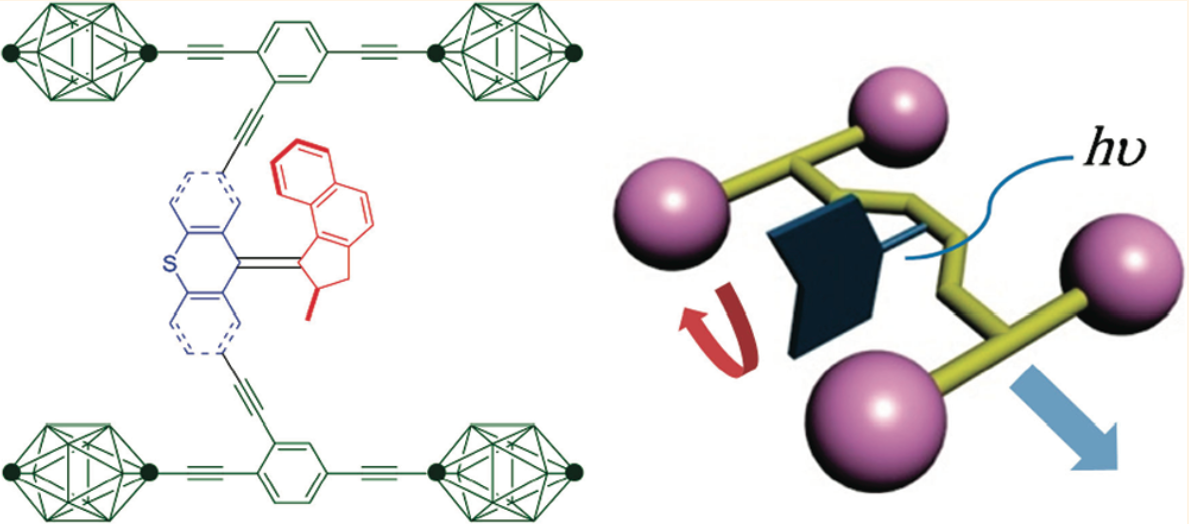
\includegraphics[width=\columnwidth]{nanocar.png}
\caption{A second generation motorized nonacar was designed, synthesized and imaged\cite{TourNanocar2012}.
\label{fig:nanocar}}
\end{center}
\end{figure}
\subsection{What types of Interaction do Bio-Inspired Robot Swarms and Flocks Afford a Human?}

In this paper, Goodrich et al. see how leader, predator, and stakeholders can work when we have a human operator and he or she can influence a decentralized agent in \cite{Goodrich2012}. They show that leaders are more effective to influence the flock, but predators can divide the flock to number of sub-flocks that is leading us to better results in some problems. For switching between modes, it is possible to have a stakeholder with more than one agent. Couzin's a non-linear controller where agents make zone dependent switches between control laws. In this bio-inspired model, three zones are defined: repulsion, orientation, and attraction. When the agents are in the zone of repulsion, agents induces repulsion to get out of that zone. If the agent is not in the zone of repulsion, the attraction and/or orientation induce forces. Their future work is to see how a team of distributed humans can use decentralized human influence to manage a bio-inspired collective.

\subsection{Controllability Characterizations of Leader-Based Swarm Interactions}

In this paper, Croix et al. research role of the network topology when controlling a network of mobile robots in \cite{Croix2012}. They have found that rank of the controllability matrix and also node centrality of the leader of the network are two parameters that determine how difficult the network is for the human. They use acyclic, cycle, and complete graph and let people vote for the difficulty and also measure their performance. They found out that a configuration with a higher rank is almost always giving a better score in comparison to lower rank. And small leader node centrality is another factor showing if the network topology is easier to control or not.

\subsection{Towards Human Control of Robot Swarms}

In this paper, Kolling et al. compare two different approaches for human operator to control the swarm: \emph{selection} and \emph{beacon} and autonomous swarm with regard to performance, adaption to complex environments, and scalability in \cite{Lewis2012}. Selection requires active selection of groups and beacon exerts a passive influence on nearby robots. They have shown that autonomous swarms have higher performance in open environments. However; selection control works better in complex environments and beacon control has a potential for scaling when we have larger swarms. 
\begin{figure}[h]
\begin{center}
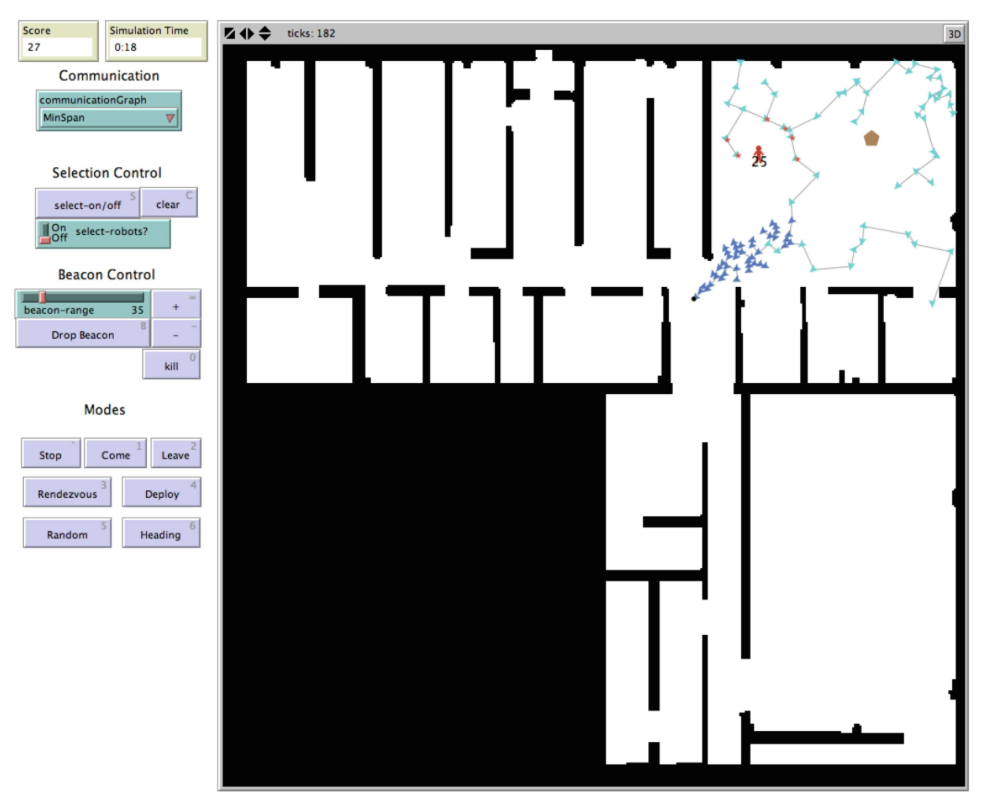
\includegraphics[width=\columnwidth]{Kolling.png}
\caption{The simple user interface used for experiments\cite{Lewis2012}.
\label{fig:kolling}}
\end{center}
\end{figure}
 
\bibliographystyle{IEEEtran}
\bibliography{LiteratureReviewShivaShahrokhi.bib}


\end{document}

 